\chapter{研究方法}

Big Little Decoder(BiLD)\upcite{kim2023speculative} 框架由 2 个解码器模型(大模型和小模型)组成,它们协同工作生成文本序列。其中,小模型运行开销小,自回归地生成大部分文本。大模型偶尔修正小模型不准确的预测,执行高效的非自回归运算。与常规的自回归执行相比,这种自回归小模型、非自回归大模型结合的方案大大提升了推理速度,最高可达原来的 2 倍,同时保持了类似或更好的生成质量。BiLD 框架可应用于各种文本生成场景,除了添加小模型外,无需进行额外的训练或修改现有的模型架构。

\begin{figure}[htbp]
    \centering
    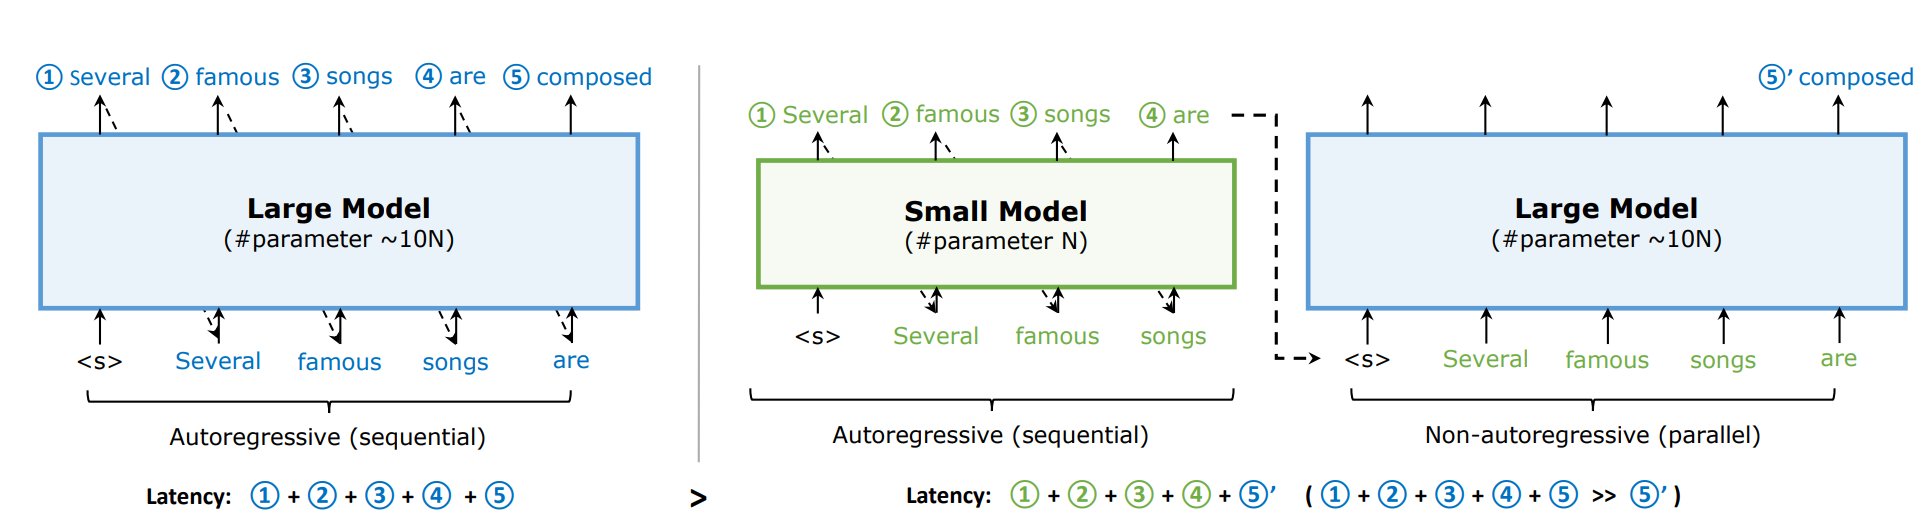
\includegraphics[width=0.9\textwidth]{BiLD.png}
    \caption{BiLD 框架}
    \label{fig:BilD}
\end{figure}

\section{可行性分析}

在多数文本生成场景中,只要纠正了部分错误预测,比大模型小一个数量级的模型也能达到与大模型相当的生成质量。为了验证这一说法,评估两种不同的生成场景:在 WMT 2014 De-En\upcite{bojar-etal-2014-findings} 上使用 mT5\upcite{xue2021mt5} 进行机器翻译,在 CNN/DailyMail\upcite{NIPS2015_afdec700} 上使用 T5\upcite{DBLP:journals/corr/abs-1910-10683} 进行机器翻译。通过控制阈值调整大模型的比重,统计大模型和小模型预测同一标记的似然性。

图~\ref*{fig:Motivating} 显示了在 2 个基准验证数据集上不同比例的大模型参与时的文本生成质量。结果表明,当大模型替代了小模型约 20\% 的不准确预测时,规模仅大模型 $1/10$ 的小模型才能保持大模型的生成质量。虽然这个实验假定大模型的预测在每次迭代中都是准确的,但它仍然证明了在保持小模型低推理延迟的同时实现大模型文本生成质量的可行性。

\begin{figure}[htbp]
    \centering
    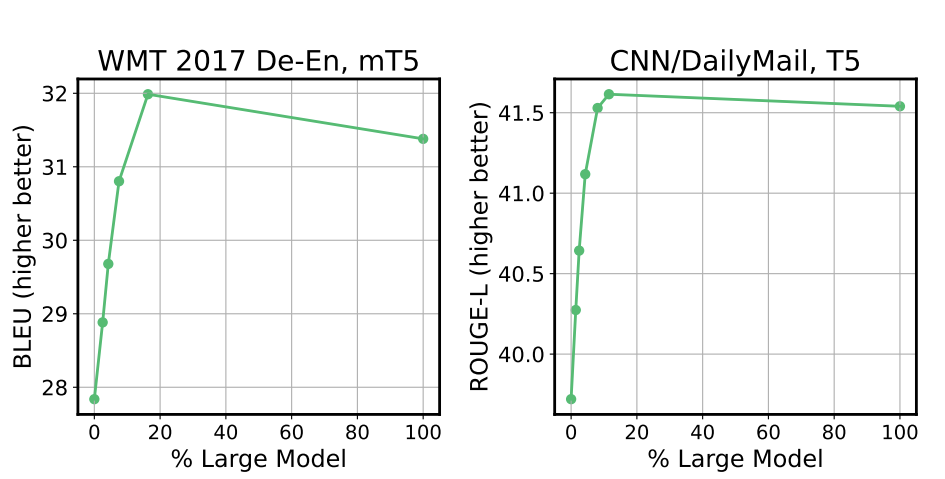
\includegraphics[width=0.9\textwidth]{Motivating.png}
    \caption{模型参与比例}
    \label{fig:Motivating}
\end{figure}

\section{Fallback 策略}

小模型需要决定何时将控制权转交给大模型。文章使用最大预测概率量化判别转交时机:当最大预测概率 $\max _y p_S\left(y \mid y_{1: n-1}\right)$ 小于阈值 $\alpha_{FB}$ 时,Fallback 使用大模型生成下一个标记。

\begin{figure}[htbp]
    \centering
    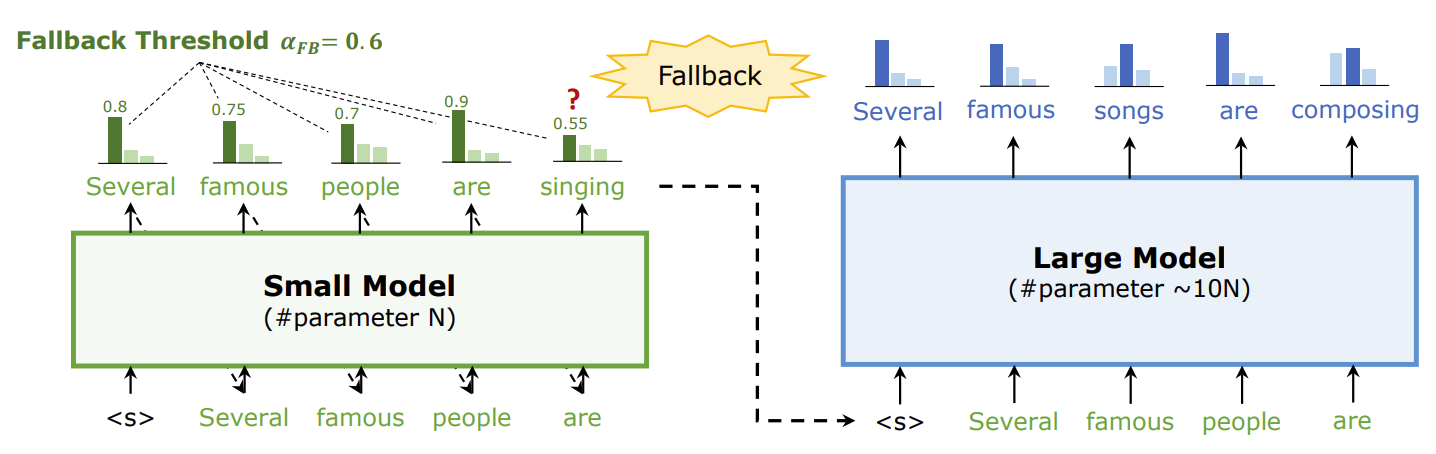
\includegraphics[width=0.9\textwidth]{Fallback.png}
    \caption{Fallback 策略}
    \label{fig:Fallback}
\end{figure}

\section{Rollback 策略}

当小模型对预测结果不够自信,决定使用 Fallback 策略时,它先前的预测可能也是不准确的。早期解码迭代中的一次错误预测会影响所有后续的文本生成,这可能大幅降低生成质量\upcite{schuster2022confident}。因此,大模型需要回顾验证小模型的历史预测,并在必要时予以修正。

对于距离指标 $d(\cdot,\cdot)$(可使用交叉熵函数),寻找大于阈值 $\alpha_{RB}$ 的最小的解码步 $m$,满足

\begin{equation}
    d\left(p_S\left(y \mid y_{1: m}\right), p_L\left(y \mid y_{1: m}\right)\right)>\alpha_{R B}
\end{equation}

如果 $m$ 存在,我们就认为小模型生成的标记 $y_m$ 是不准确的,Rollback 撤销 $y_{m}$ 和 $y_{n}$ 之间的预测并将 $y_m$ 替换为大模型的预测 $y_{m,L}$。

\begin{figure}[htbp]
    \centering
    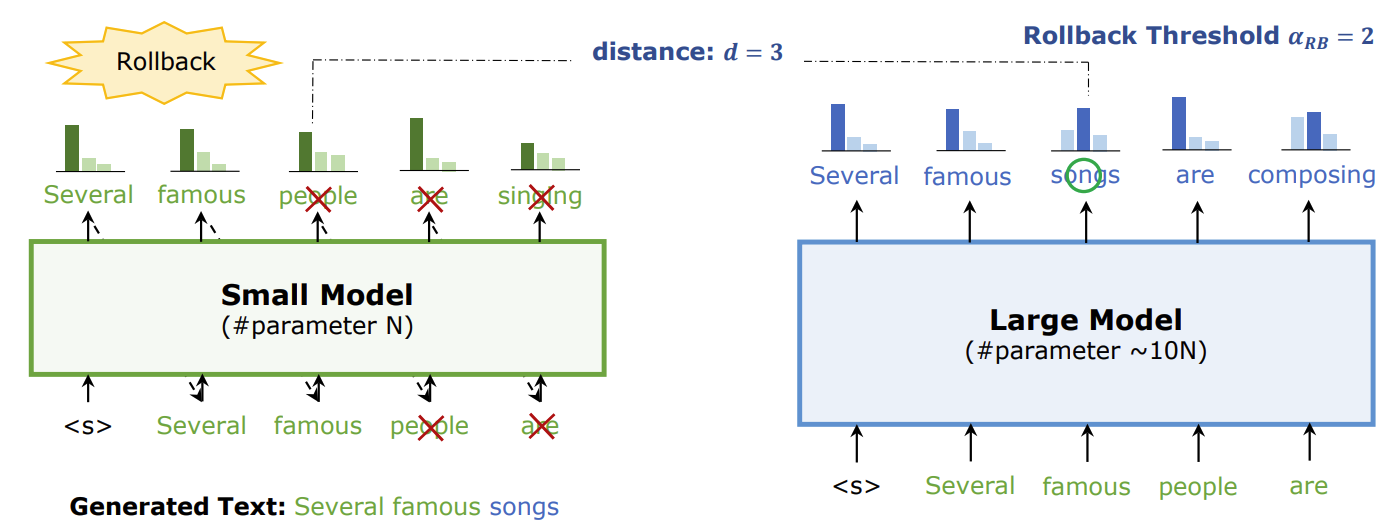
\includegraphics[width=0.9\textwidth]{Rollback.png}
    \caption{Rollback 策略}
    \label{fig:Rollback}
\end{figure}

\section{预测对齐}

如果大模型和小模型的词汇表一致,BiLD 框架对大小模型的选择没有限制。然而,当两个模型分别训练时,他们可能会得到语义相近但是词汇表不同的训练结果。Rollback 策略需要衡量大模型和小模型的标记相似度,语义相近但是词汇不同的标记会造成额外的 Rollback,这样非但不会提升生成质量,还会降低推理速度。

为了对齐小模型和大模型的词汇表,BiLD 可以使用模型对齐技术。在使用数据集训练完大模型后,提取一个能有效表示数据集语句分布的校准数据集 $\mathcal{X}_{\mathrm{cal}}=\{x^{(i)}\}$,使用大模型获取对应的输出 $\mathcal{Y}_{\mathrm{cal}}=\{y^{(i)}\}$。再使用校准集 $\left(x_{\mathrm{cal}}, y_{\mathrm{cal}}\right) \in\left(\mathcal{X}_{\mathrm{cal}}, \mathcal{Y}_{\mathrm{cal}}\right)$ 对小模型进行微调。

这样做可以提升小模型和大模型的预测相似度,降低 Rollback 判断中的距离 $d(\cdot,\cdot)$,从而减少不必要的 Rollback,进一步提升 BiLD 推理速度。
